\chapter{Procesos de desarrollo}
\label{chap:procesos-desarrollo}

\par Un proceso de desarrollo en el mundo del software se define como:

\begin{quote}
\emph{El proceso de transformación de unos requerimientos en una solución. Un conjunto de pautas a seguir para completar el ciclo de vida de la solución de una manera organizada, sistemática y que ayude a las personas a completar los objetivos fijados}
\end{quote}

\par En SidelabCode Stack se optó por implementar el proceso de desarrollo de software \emph{iterativo e incremental} para crear el dise\~no de la forja SidelabCode Stack a través de metodolog\'ias ágiles.

\par El proceso de desarrollo infiere directamente en la calidad del software que se construye. Es la parte más importante en el software ya que un proceso de desarrollo óptimo para una solución otorga las herramientas necesarias para una mejor evolución del mismo. Cada proceso de desarrollo ha de aplicarse a la solución según los requisitos de la misma, no todos los procesos de desarrollo son válidos para todos los proyectos.

\section{Software de Calidad}
\label{sec:software-calidad}

\par Desarrollar Software de Calidad, para ellos nos encontramos con la palabra \emph{"Calidad"} tan subjetiva en muchos ámbitos, pero que en el desarrollo puede ser bastante objetiva ya que se trata de Software, una ciencia evaluable. La Calidad del Software es el conjunto de cualidades que lo caracterizan y determinan su viabilidad y utilidad; Mantenibilidad, Fiable, Eficiencia y Seguridad.

\begin{figure}[H]
    \begin{center}	
        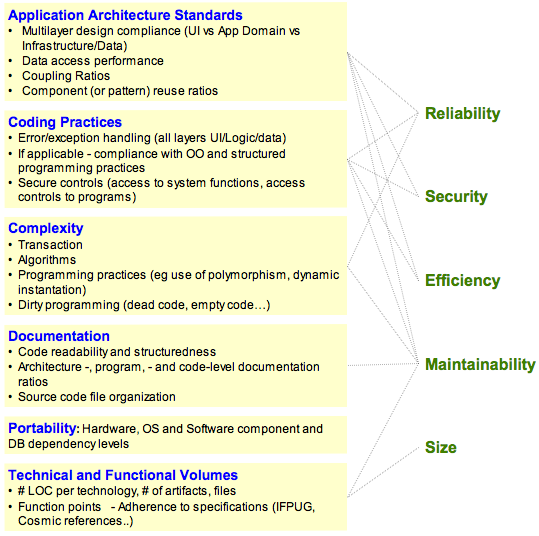
\includegraphics[width=0.7\textwidth]{SoftwareQuality}
        \caption{Software de Calidad}
        \label{fig:softwarequality}
    \end{center}
\end{figure}

\par Un software hecho para ejecutarse una sola vez no requiere el mismo nivel de calidad mientras que un software para ser explotado durante un largo necesita ser fiable, seguro, mantenible y flexible para disminuir los costes.

\begin{itemize}
	\item \emph{Mantenibilidad}: El software debe ser diseñado de tal manera, que permita ajustarlo a los cambios en los requerimientos. Esta característica es crucial, debido al inevitable cambio del contexto en el que se desempeña un software.
	\item \emph{Fiabilidad}: Incluye varias características además de la fiabilidad, como la aplicación de estándares, complejidad, tratamiento de errores.
	\item \emph{Eficiencia}: Tiene que ver con el uso eficiente de los recursos que necesita un sistema para su funcionamiento.
	\item \emph{Seguridad}: La evaluación de la seguridad requiere un control sobre la arquitectura, el diseño y las buenas prácticas.
\end{itemize}

% section software-calidad (end)

\section{Proceso iterativo}
\label{sec:proc-iterativo}

\par ¿ Que es el proceso iterativo ?

\begin{quote}
    \emph{La primera versión debe contener todos los requerimientos del usuario y lo que se va a hacer en las siguientes versiones es ir mejorando aspectos como la funcionalidad o el tiempo de respuesta.}\footnote{Procesos Iterativos e Incrementales - \url{http://esalas334.blogspot.es/1193761920/}}
\end{quote}

\par Se centra más en la inmediatez de la primera versión y en las mejoras posteriores que se van creando enfocadas a la solución final. En el proceso también juega una parte fundamental la comunicación con el cliente a través de la visualización de los resultados por iteraciones. De esta forma se consigue una buena coordinación entre el cliente y el equipo de desarrollo para la consecución de los objetivos. Teniendo en cuenta posibles cambios entre iteraciones pero nunca del resultado completo, así controlando a tiempo la \emph{desviación} que pueda existir en el proceso de la creación de producto.

\begin{quote}
    \emph{Como la idea que representa la palabra iterativo, un proceso de desarrollo de software iterativo es aquel al que se lo piensa, como una serie de tareas agrupadas en pequeñas etapas repetitivas. Estas "pequeñas etapas repetitivas" son las iteraciones.}\footnote{Proceso de Desarrollo Iterativo - Fernando Soriano - \url{http://fernandosoriano.com.ar/?p=13}}
\end{quote}

\par La base el proceso de desarrollo Iterativo provee un conjunto de pasos para el desarrollo de la solución que se repiten iteración tras iteración para la creación de mejoras tangibles y/o evaluables. 

\begin{figure}[htp]
    \centering
    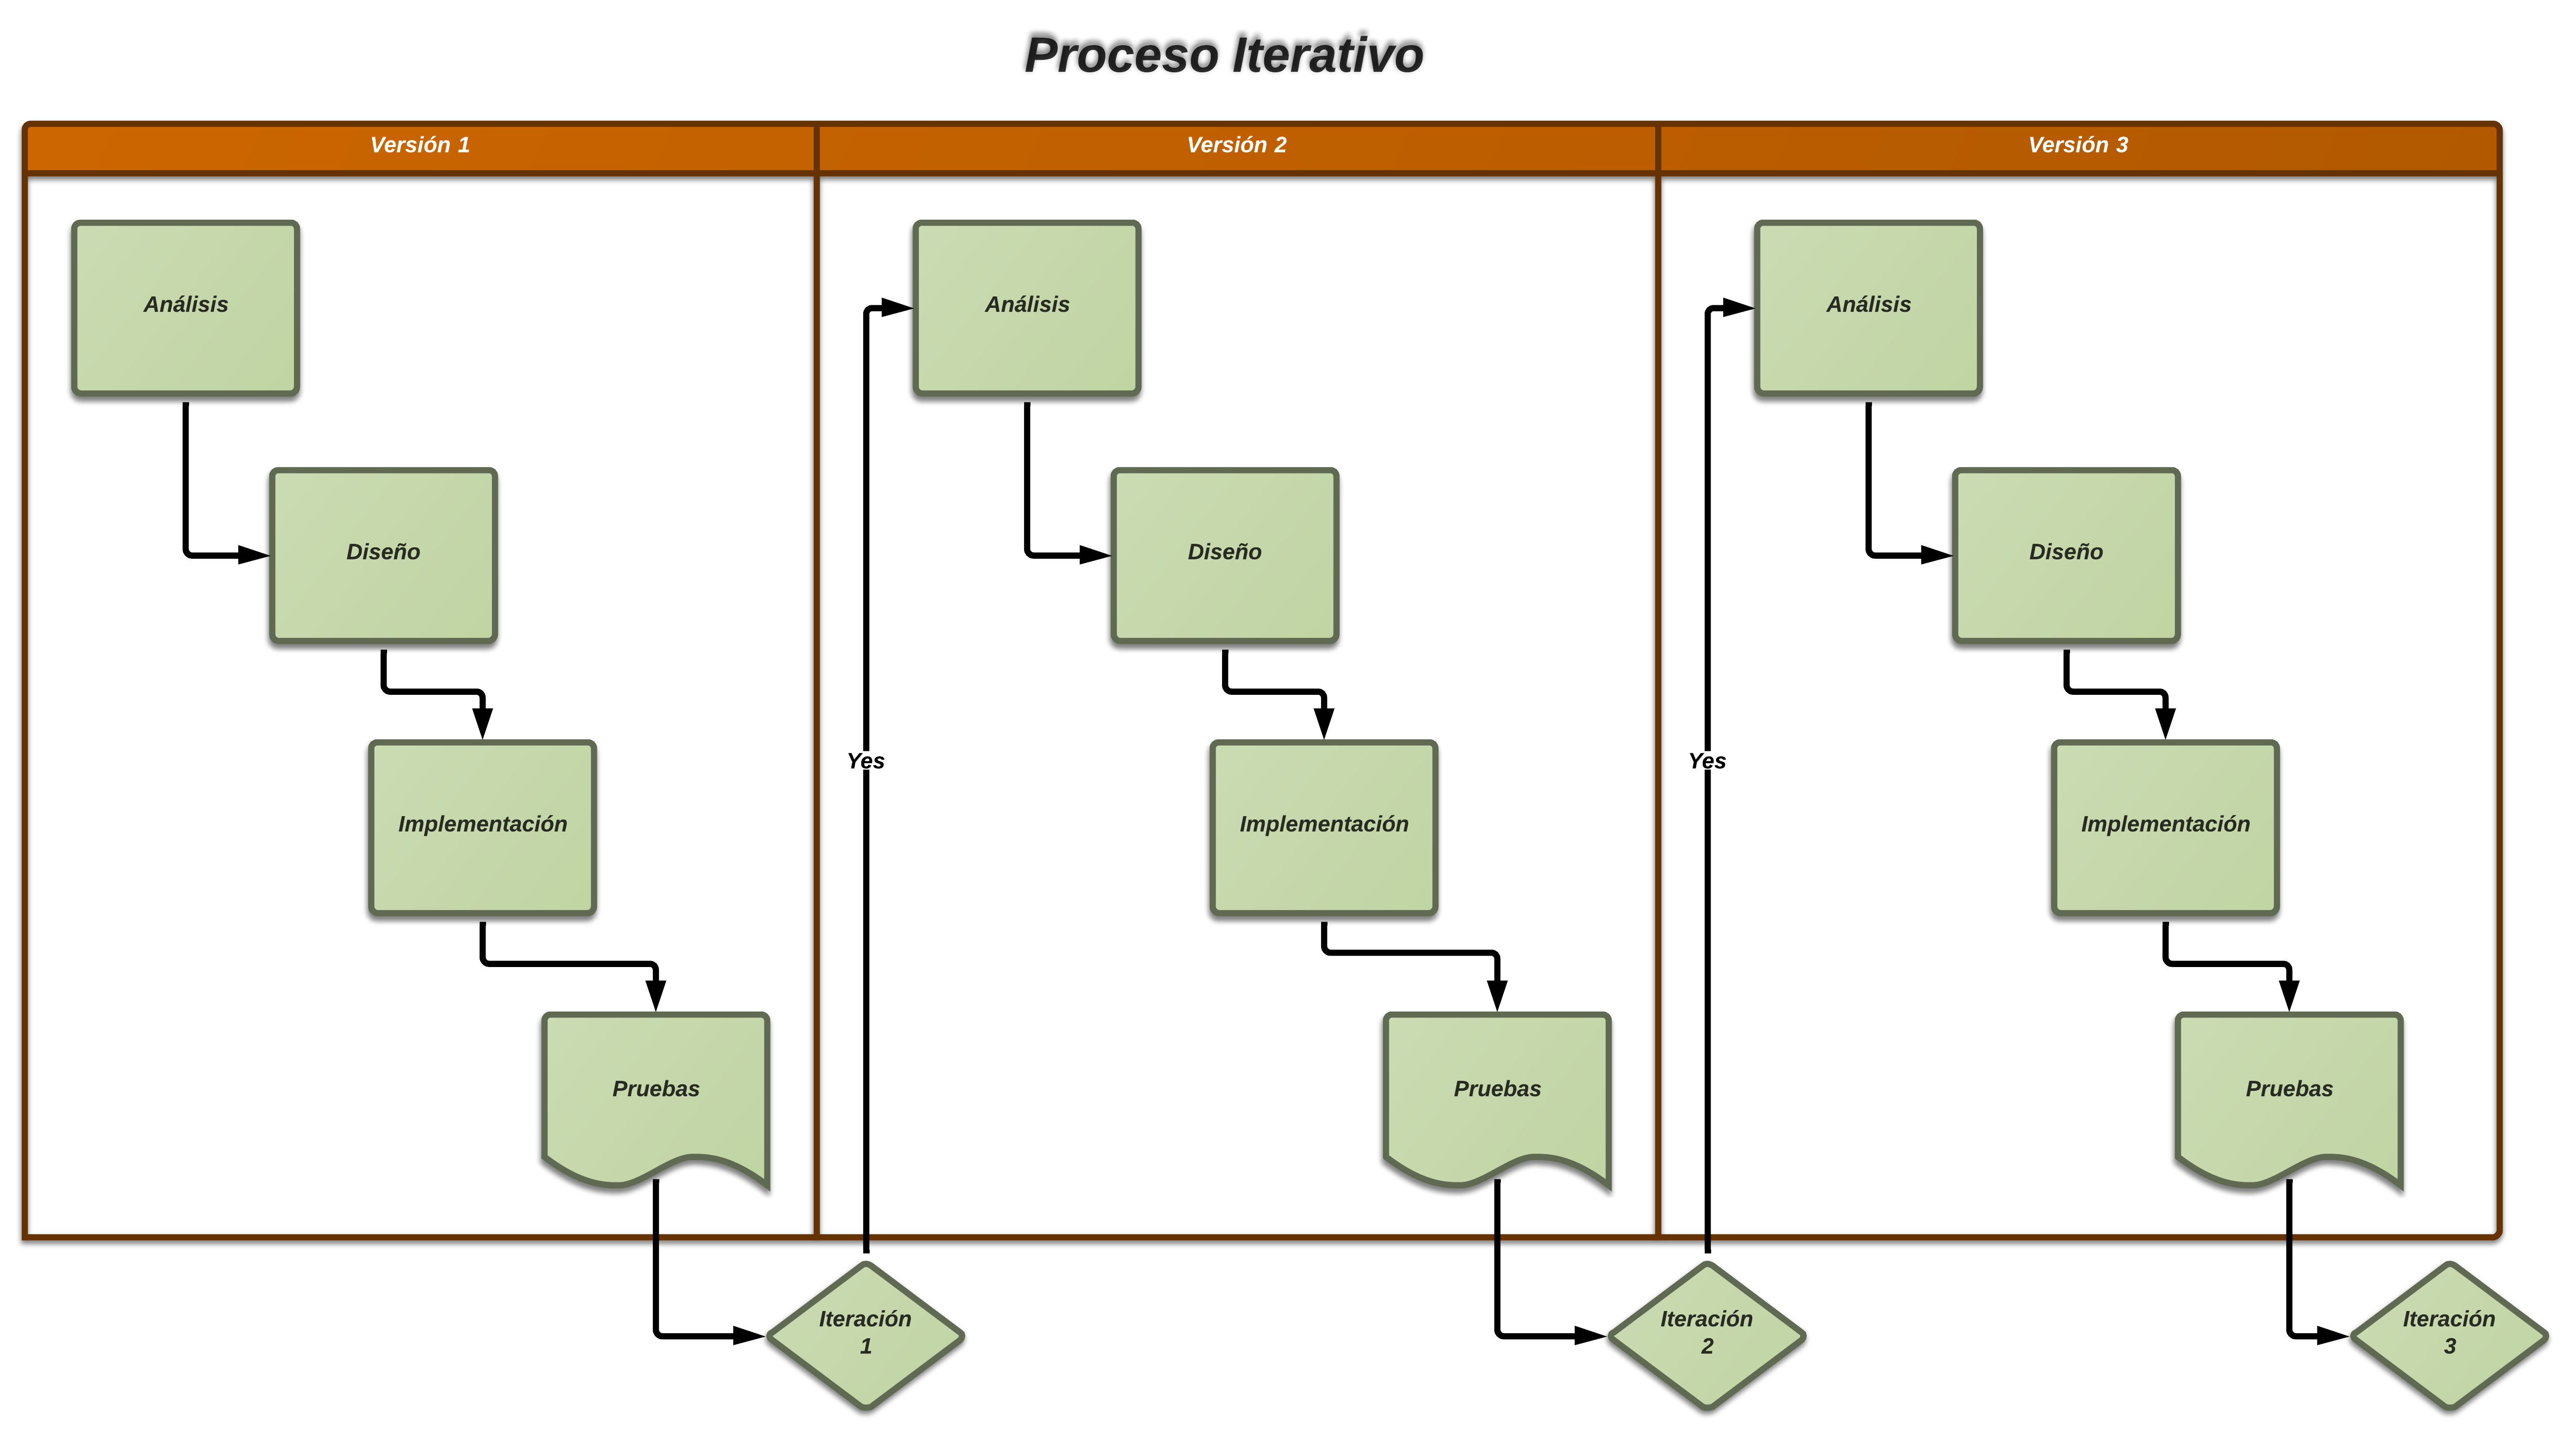
\includegraphics[width=1\textwidth]{ProcesoIterativo}
    \caption{Proceso Iterativo}
    \label{fig:ProcesoIterativo}
\end{figure}

\par En cada iteración se construye una pieza funcional del producto final, completa, testeada, documentada e integrada en la solución final. La visión completa de este proceso muestra una línea de iteraciones separadas funcionalmente unas de otras que en conjunto, forman la solución final. Iteraciones independientes unas de otras a través de un desarrollo lineal agrupando pequeños ciclos de desarrollo.

\begin{itemize}
	\item \emph{Duración fija}, quiere decir que una vez establecidos los tiempos o planificación de la iteración, la iteración termina en la fecha exacta establecida. Si el equipo no pudo cumplir lo planificado, el desarrollo pendiente pasa a otra iteración.
	\item Estimación de tiempos cortos, las \emph{"buenas prácticas"} hablan de que una iteración debiera durar entre 2 y 6 semanas.
	\item Es como un ciclo de desarrollo completo, ya que en una iteración se realizan actividades de análisis, diseño, implementación, pruebas, etc.
\end{itemize}

% section proc-iterativo (end)

\section{Proceso incremental}
\label{sec:proc-incremental}

% section proc-incremental (end)

\section{Iterativo e Incremental}
\label{sec:iterativo-incremental}

Desarrollo iterativo e incremental

% section iterativo-incremental (end)
\section{Gestión de tareas}
\label{sec:gestion-tareas}

\par Gestión de tareas: ¿qué hay que hacer? ¿quién tiene que hacerlo? -> Sistemas de gestión de tickets
% section gestion-tareas (end)

\section{Código versionado}
\label{sec:codigo-versionado}

\par Código versionado -> repositorios de código

% section codigo-versionado (end)

\section{TDD y CI}
\label{sec:tdd-ci}

\par TDD -> sistemas de CI para asegurar que los tests se pasan regularmente

% section tdd-ci (end)

\section{Desarrollo por canales}
\label{sec:desarrollo-canales}

% section desarrollo-canales (end)

\section{Herramientas}
\label{sec:herramientas}

% section herramientas (end)
